\documentclass[aspectratio=1610]{beamer}
\usepackage[utf8]{inputenc}
% \usepackage[default,oldstyle,scale=0.95]{opensans}
% \usepackage[T1]{fontenc}
\usepackage{sansmathfonts}
\usepackage[T1]{fontenc}

\usepackage[natbib=true,style=numeric,sorting=none]{biblatex}
\addbibresource{references.bib}

\usepackage{tikz}
\usepackage{tikz-3dplot}

\usepackage{pgf-pie}  
\usepackage{caption}
\usepackage{subcaption}
\usepackage{algorithm}
\usepackage{algpseudocode}
\usepackage{amsmath,amssymb,amsfonts}
\usepackage{svg}

\usetikzlibrary{arrows.meta}
\usetikzlibrary{tikzmark}
\usetikzlibrary{math}
\usetikzlibrary{backgrounds,calc,positioning}
\usepackage{qrcode}
\usepackage{siunitx}
\usetikzlibrary{patterns,positioning,arrows.meta,decorations.pathreplacing}

\usepackage{pgfplots}
\usepackage{algorithm, algpseudocode}



\usetheme{main}

\captionsetup{font=scriptsize,labelfont=scriptsize}


\title[Numerical optimization]{Numerical optimization : theory and applications}

\date[]{}
\author[AM]{\textbf{Ammar Mian} \\ \footnotesize Associate professor, LISTIC, Université Savoie Mont Blanc}

\newcommand{\red}[1]{\textcolor{red}{#1}}
% \newcommand{\alert}[1]{{\textbf{\alert{#1}}}}


%%%%%% NEW MATH DEFINITIONS %%%%%

\usepackage{amsmath,amsfonts,bm}

% Mark sections of captions for referring to divisions of figures
\newcommand{\figleft}{{\em (Left)}}
\newcommand{\figcenter}{{\em (Center)}}
\newcommand{\figright}{{\em (Right)}}
\newcommand{\figtop}{{\em (Top)}}
\newcommand{\figbottom}{{\em (Bottom)}}
\newcommand{\captiona}{{\em (a)}}
\newcommand{\captionb}{{\em (b)}}
\newcommand{\captionc}{{\em (c)}}
\newcommand{\captiond}{{\em (d)}}

% Highlight a newly defined term
\newcommand{\newterm}[1]{{\bf #1}}


% Figure reference, lower-case.
\def\figref#1{figure~\ref{#1}}
% Figure reference, capital. For start of sentence
\def\Figref#1{Figure~\ref{#1}}
\def\twofigref#1#2{figures \ref{#1} and \ref{#2}}
\def\quadfigref#1#2#3#4{figures \ref{#1}, \ref{#2}, \ref{#3} and \ref{#4}}
% Section reference, lower-case.
\def\secref#1{section~\ref{#1}}
% Section reference, capital.
\def\Secref#1{Section~\ref{#1}}
% Reference to two sections.
\def\twosecrefs#1#2{sections \ref{#1} and \ref{#2}}
% Reference to three sections.
\def\secrefs#1#2#3{sections \ref{#1}, \ref{#2} and \ref{#3}}
% Reference to an equation, lower-case.
% \def\eqref#1{equation~\ref{#1}}
% Reference to an equation, upper case
\def\Eqref#1{Equation~\ref{#1}}
% A raw reference to an equation---avoid using if possible
\def\plaineqref#1{\ref{#1}}
% Reference to a chapter, lower-case.
\def\chapref#1{chapter~\ref{#1}}
% Reference to an equation, upper case.
\def\Chapref#1{Chapter~\ref{#1}}
% Reference to a range of chapters
\def\rangechapref#1#2{chapters\ref{#1}--\ref{#2}}
% Reference to an algorithm, lower-case.
\def\algref#1{algorithm~\ref{#1}}
% Reference to an algorithm, upper case.
\def\Algref#1{Algorithm~\ref{#1}}
\def\twoalgref#1#2{algorithms \ref{#1} and \ref{#2}}
\def\Twoalgref#1#2{Algorithms \ref{#1} and \ref{#2}}
% Reference to a part, lower case
\def\partref#1{part~\ref{#1}}
% Reference to a part, upper case
\def\Partref#1{Part~\ref{#1}}
\def\twopartref#1#2{parts \ref{#1} and \ref{#2}}

\def\ceil#1{\lceil #1 \rceil}
\def\floor#1{\lfloor #1 \rfloor}
\def\1{\bm{1}}
\newcommand{\train}{\mathcal{D}}
\newcommand{\valid}{\mathcal{D_{\mathrm{valid}}}}
\newcommand{\test}{\mathcal{D_{\mathrm{test}}}}

\def\eps{{\epsilon}}


% Random variables
\def\reta{{\textnormal{$\eta$}}}
\def\ra{{\textnormal{a}}}
\def\rb{{\textnormal{b}}}
\def\rc{{\textnormal{c}}}
\def\rd{{\textnormal{d}}}
\def\re{{\textnormal{e}}}
\def\rf{{\textnormal{f}}}
\def\rg{{\textnormal{g}}}
\def\rh{{\textnormal{h}}}
\def\ri{{\textnormal{i}}}
\def\rj{{\textnormal{j}}}
\def\rk{{\textnormal{k}}}
\def\rl{{\textnormal{l}}}
% rm is already a command, just don't name any random variables m
\def\rn{{\textnormal{n}}}
\def\ro{{\textnormal{o}}}
\def\rp{{\textnormal{p}}}
\def\rq{{\textnormal{q}}}
\def\rr{{\textnormal{r}}}
\def\rs{{\textnormal{s}}}
\def\rt{{\textnormal{t}}}
\def\ru{{\textnormal{u}}}
\def\rv{{\textnormal{v}}}
\def\rw{{\textnormal{w}}}
\def\rx{{\textnormal{x}}}
\def\ry{{\textnormal{y}}}
\def\rz{{\textnormal{z}}}

% Random vectors
\def\rvepsilon{{\mathbf{\epsilon}}}
\def\rvtheta{{\mathbf{\theta}}}
\def\rva{{\mathbf{a}}}
\def\rvb{{\mathbf{b}}}
\def\rvc{{\mathbf{c}}}
\def\rvd{{\mathbf{d}}}
\def\rve{{\mathbf{e}}}
\def\rvf{{\mathbf{f}}}
\def\rvg{{\mathbf{g}}}
\def\rvh{{\mathbf{h}}}
\def\rvu{{\mathbf{i}}}
\def\rvj{{\mathbf{j}}}
\def\rvk{{\mathbf{k}}}
\def\rvl{{\mathbf{l}}}
\def\rvm{{\mathbf{m}}}
\def\rvn{{\mathbf{n}}}
\def\rvo{{\mathbf{o}}}
\def\rvp{{\mathbf{p}}}
\def\rvq{{\mathbf{q}}}
\def\rvr{{\mathbf{r}}}
\def\rvs{{\mathbf{s}}}
\def\rvt{{\mathbf{t}}}
\def\rvu{{\mathbf{u}}}
\def\rvv{{\mathbf{v}}}
\def\rvw{{\mathbf{w}}}
\def\rvx{{\mathbf{x}}}
\def\rvy{{\mathbf{y}}}
\def\rvz{{\mathbf{z}}}

% Elements of random vectors
\def\erva{{\textnormal{a}}}
\def\ervb{{\textnormal{b}}}
\def\ervc{{\textnormal{c}}}
\def\ervd{{\textnormal{d}}}
\def\erve{{\textnormal{e}}}
\def\ervf{{\textnormal{f}}}
\def\ervg{{\textnormal{g}}}
\def\ervh{{\textnormal{h}}}
\def\ervi{{\textnormal{i}}}
\def\ervj{{\textnormal{j}}}
\def\ervk{{\textnormal{k}}}
\def\ervl{{\textnormal{l}}}
\def\ervm{{\textnormal{m}}}
\def\ervn{{\textnormal{n}}}
\def\ervo{{\textnormal{o}}}
\def\ervp{{\textnormal{p}}}
\def\ervq{{\textnormal{q}}}
\def\ervr{{\textnormal{r}}}
\def\ervs{{\textnormal{s}}}
\def\ervt{{\textnormal{t}}}
\def\ervu{{\textnormal{u}}}
\def\ervv{{\textnormal{v}}}
\def\ervw{{\textnormal{w}}}
\def\ervx{{\textnormal{x}}}
\def\ervy{{\textnormal{y}}}
\def\ervz{{\textnormal{z}}}

% Random matrices
\def\rmA{{\mathbf{A}}}
\def\rmB{{\mathbf{B}}}
\def\rmC{{\mathbf{C}}}
\def\rmD{{\mathbf{D}}}
\def\rmE{{\mathbf{E}}}
\def\rmF{{\mathbf{F}}}
\def\rmG{{\mathbf{G}}}
\def\rmH{{\mathbf{H}}}
\def\rmI{{\mathbf{I}}}
\def\rmJ{{\mathbf{J}}}
\def\rmK{{\mathbf{K}}}
\def\rmL{{\mathbf{L}}}
\def\rmM{{\mathbf{M}}}
\def\rmN{{\mathbf{N}}}
\def\rmO{{\mathbf{O}}}
\def\rmP{{\mathbf{P}}}
\def\rmQ{{\mathbf{Q}}}
\def\rmR{{\mathbf{R}}}
\def\rmS{{\mathbf{S}}}
\def\rmT{{\mathbf{T}}}
\def\rmU{{\mathbf{U}}}
\def\rmV{{\mathbf{V}}}
\def\rmW{{\mathbf{W}}}
\def\rmX{{\mathbf{X}}}
\def\rmY{{\mathbf{Y}}}
\def\rmZ{{\mathbf{Z}}}

% Elements of random matrices
\def\ermA{{\textnormal{A}}}
\def\ermB{{\textnormal{B}}}
\def\ermC{{\textnormal{C}}}
\def\ermD{{\textnormal{D}}}
\def\ermE{{\textnormal{E}}}
\def\ermF{{\textnormal{F}}}
\def\ermG{{\textnormal{G}}}
\def\ermH{{\textnormal{H}}}
\def\ermI{{\textnormal{I}}}
\def\ermJ{{\textnormal{J}}}
\def\ermK{{\textnormal{K}}}
\def\ermL{{\textnormal{L}}}
\def\ermM{{\textnormal{M}}}
\def\ermN{{\textnormal{N}}}
\def\ermO{{\textnormal{O}}}
\def\ermP{{\textnormal{P}}}
\def\ermQ{{\textnormal{Q}}}
\def\ermR{{\textnormal{R}}}
\def\ermS{{\textnormal{S}}}
\def\ermT{{\textnormal{T}}}
\def\ermU{{\textnormal{U}}}
\def\ermV{{\textnormal{V}}}
\def\ermW{{\textnormal{W}}}
\def\ermX{{\textnormal{X}}}
\def\ermY{{\textnormal{Y}}}
\def\ermZ{{\textnormal{Z}}}

% Vectors
\def\vzero{{\bm{0}}}
\def\vone{{\bm{1}}}
\def\vmu{{\bm{\mu}}}
\def\vtheta{{\bm{\theta}}}
\def\va{{\bm{a}}}
\def\vb{{\bm{b}}}
\def\vc{{\bm{c}}}
\def\vd{{\bm{d}}}
\def\ve{{\bm{e}}}
\def\vf{{\bm{f}}}
\def\vg{{\bm{g}}}
\def\vh{{\bm{h}}}
\def\vi{{\bm{i}}}
\def\vj{{\bm{j}}}
\def\vk{{\bm{k}}}
\def\vl{{\bm{l}}}
\def\vm{{\bm{m}}}
\def\vn{{\bm{n}}}
\def\vo{{\bm{o}}}
\def\vp{{\bm{p}}}
\def\vq{{\bm{q}}}
\def\vr{{\bm{r}}}
\def\vs{{\bm{s}}}
\def\vt{{\bm{t}}}
\def\vu{{\bm{u}}}
\def\vv{{\bm{v}}}
\def\vw{{\bm{w}}}
\def\vx{{\bm{x}}}
\def\vy{{\bm{y}}}
\def\vz{{\bm{z}}}

% Elements of vectors
\def\evalpha{{\alpha}}
\def\evbeta{{\beta}}
\def\evepsilon{{\epsilon}}
\def\evlambda{{\lambda}}
\def\evomega{{\omega}}
\def\evmu{{\mu}}
\def\evpsi{{\psi}}
\def\evsigma{{\sigma}}
\def\evtheta{{\theta}}
\def\eva{{a}}
\def\evb{{b}}
\def\evc{{c}}
\def\evd{{d}}
\def\eve{{e}}
\def\evf{{f}}
\def\evg{{g}}
\def\evh{{h}}
\def\evi{{i}}
\def\evj{{j}}
\def\evk{{k}}
\def\evl{{l}}
\def\evm{{m}}
\def\evn{{n}}
\def\evo{{o}}
\def\evp{{p}}
\def\evq{{q}}
\def\evr{{r}}
\def\evs{{s}}
\def\evt{{t}}
\def\evu{{u}}
\def\evv{{v}}
\def\evw{{w}}
\def\evx{{x}}
\def\evy{{y}}
\def\evz{{z}}

% Matrix
\def\mA{{\bm{A}}}
\def\mB{{\bm{B}}}
\def\mC{{\bm{C}}}
\def\mD{{\bm{D}}}
\def\mE{{\bm{E}}}
\def\mF{{\bm{F}}}
\def\mG{{\bm{G}}}
\def\mH{{\bm{H}}}
\def\mI{{\bm{I}}}
\def\mJ{{\bm{J}}}
\def\mK{{\bm{K}}}
\def\mL{{\bm{L}}}
\def\mM{{\bm{M}}}
\def\mN{{\bm{N}}}
\def\mO{{\bm{O}}}
\def\mP{{\bm{P}}}
\def\mQ{{\bm{Q}}}
\def\mR{{\bm{R}}}
\def\mS{{\bm{S}}}
\def\mT{{\bm{T}}}
\def\mU{{\bm{U}}}
\def\mV{{\bm{V}}}
\def\mW{{\bm{W}}}
\def\mX{{\bm{X}}}
\def\mY{{\bm{Y}}}
\def\mZ{{\bm{Z}}}
\def\mBeta{{\bm{\beta}}}
\def\mPhi{{\bm{\Phi}}}
\def\mLambda{{\bm{\Lambda}}}
\def\mSigma{{\bm{\Sigma}}}

% Tensor
\DeclareMathAlphabet{\mathsfit}{\encodingdefault}{\sfdefault}{m}{sl}
\SetMathAlphabet{\mathsfit}{bold}{\encodingdefault}{\sfdefault}{bx}{n}
\newcommand{\tens}[1]{\bm{\mathsfit{#1}}}
\def\tA{{\tens{A}}}
\def\tB{{\tens{B}}}
\def\tC{{\tens{C}}}
\def\tD{{\tens{D}}}
\def\tE{{\tens{E}}}
\def\tF{{\tens{F}}}
\def\tG{{\tens{G}}}
\def\tH{{\tens{H}}}
\def\tI{{\tens{I}}}
\def\tJ{{\tens{J}}}
\def\tK{{\tens{K}}}
\def\tL{{\tens{L}}}
\def\tM{{\tens{M}}}
\def\tN{{\tens{N}}}
\def\tO{{\tens{O}}}
\def\tP{{\tens{P}}}
\def\tQ{{\tens{Q}}}
\def\tR{{\tens{R}}}
\def\tS{{\tens{S}}}
\def\tT{{\tens{T}}}
\def\tU{{\tens{U}}}
\def\tV{{\tens{V}}}
\def\tW{{\tens{W}}}
\def\tX{{\tens{X}}}
\def\tY{{\tens{Y}}}
\def\tZ{{\tens{Z}}}


% Graph
\def\gA{{\mathcal{A}}}
\def\gB{{\mathcal{B}}}
\def\gC{{\mathcal{C}}}
\def\gD{{\mathcal{D}}}
\def\gE{{\mathcal{E}}}
\def\gF{{\mathcal{F}}}
\def\gG{{\mathcal{G}}}
\def\gH{{\mathcal{H}}}
\def\gI{{\mathcal{I}}}
\def\gJ{{\mathcal{J}}}
\def\gK{{\mathcal{K}}}
\def\gL{{\mathcal{L}}}
\def\gM{{\mathcal{M}}}
\def\gN{{\mathcal{N}}}
\def\gO{{\mathcal{O}}}
\def\gP{{\mathcal{P}}}
\def\gQ{{\mathcal{Q}}}
\def\gR{{\mathcal{R}}}
\def\gS{{\mathcal{S}}}
\def\gT{{\mathcal{T}}}
\def\gU{{\mathcal{U}}}
\def\gV{{\mathcal{V}}}
\def\gW{{\mathcal{W}}}
\def\gX{{\mathcal{X}}}
\def\gY{{\mathcal{Y}}}
\def\gZ{{\mathcal{Z}}}

% Sets
\def\sA{{\mathbb{A}}}
\def\sB{{\mathbb{B}}}
\def\sC{{\mathbb{C}}}
\def\sD{{\mathbb{D}}}
% Don't use a set called E, because this would be the same as our symbol
% for expectation.
\def\sF{{\mathbb{F}}}
\def\sG{{\mathbb{G}}}
\def\sH{{\mathbb{H}}}
\def\sI{{\mathbb{I}}}
\def\sJ{{\mathbb{J}}}
\def\sK{{\mathbb{K}}}
\def\sL{{\mathbb{L}}}
\def\sM{{\mathbb{M}}}
\def\sN{{\mathbb{N}}}
\def\sO{{\mathbb{O}}}
\def\sP{{\mathbb{P}}}
\def\sQ{{\mathbb{Q}}}
\def\sR{{\mathbb{R}}}
\def\sS{{\mathbb{S}}}
\def\sT{{\mathbb{T}}}
\def\sU{{\mathbb{U}}}
\def\sV{{\mathbb{V}}}
\def\sW{{\mathbb{W}}}
\def\sX{{\mathbb{X}}}
\def\sY{{\mathbb{Y}}}
\def\sZ{{\mathbb{Z}}}

% Entries of a matrix
\def\emLambda{{\Lambda}}
\def\emA{{A}}
\def\emB{{B}}
\def\emC{{C}}
\def\emD{{D}}
\def\emE{{E}}
\def\emF{{F}}
\def\emG{{G}}
\def\emH{{H}}
\def\emI{{I}}
\def\emJ{{J}}
\def\emK{{K}}
\def\emL{{L}}
\def\emM{{M}}
\def\emN{{N}}
\def\emO{{O}}
\def\emP{{P}}
\def\emQ{{Q}}
\def\emR{{R}}
\def\emS{{S}}
\def\emT{{T}}
\def\emU{{U}}
\def\emV{{V}}
\def\emW{{W}}
\def\emX{{X}}
\def\emY{{Y}}
\def\emZ{{Z}}
\def\emSigma{{\Sigma}}

% entries of a tensor
% Same font as tensor, without \bm wrapper
\newcommand{\etens}[1]{\mathsfit{#1}}
\def\etLambda{{\etens{\Lambda}}}
\def\etA{{\etens{A}}}
\def\etB{{\etens{B}}}
\def\etC{{\etens{C}}}
\def\etD{{\etens{D}}}
\def\etE{{\etens{E}}}
\def\etF{{\etens{F}}}
\def\etG{{\etens{G}}}
\def\etH{{\etens{H}}}
\def\etI{{\etens{I}}}
\def\etJ{{\etens{J}}}
\def\etK{{\etens{K}}}
\def\etL{{\etens{L}}}
\def\etM{{\etens{M}}}
\def\etN{{\etens{N}}}
\def\etO{{\etens{O}}}
\def\etP{{\etens{P}}}
\def\etQ{{\etens{Q}}}
\def\etR{{\etens{R}}}
\def\etS{{\etens{S}}}
\def\etT{{\etens{T}}}
\def\etU{{\etens{U}}}
\def\etV{{\etens{V}}}
\def\etW{{\etens{W}}}
\def\etX{{\etens{X}}}
\def\etY{{\etens{Y}}}
\def\etZ{{\etens{Z}}}

% The true underlying data generating distribution
\newcommand{\pdata}{p_{\rm{data}}}
% The empirical distribution defined by the training set
\newcommand{\ptrain}{\hat{p}_{\rm{data}}}
\newcommand{\Ptrain}{\hat{P}_{\rm{data}}}
% The model distribution
\newcommand{\pmodel}{p_{\rm{model}}}
\newcommand{\Pmodel}{P_{\rm{model}}}
\newcommand{\ptildemodel}{\tilde{p}_{\rm{model}}}
% Stochastic autoencoder distributions
\newcommand{\pencode}{p_{\rm{encoder}}}
\newcommand{\pdecode}{p_{\rm{decoder}}}
\newcommand{\precons}{p_{\rm{reconstruct}}}

\newcommand{\laplace}{\mathrm{Laplace}} % Laplace distribution

\newcommand{\E}{\mathbb{E}}
\newcommand{\Ls}{\mathcal{L}}
% \newcommand{\R}{\mathbb{R}}
\newcommand{\emp}{\tilde{p}}
\newcommand{\lr}{\alpha}
\newcommand{\reg}{\lambda}
\newcommand{\rect}{\mathrm{rectifier}}
\newcommand{\softmax}{\mathrm{softmax}}
\newcommand{\sigmoid}{\sigma}
\newcommand{\softplus}{\zeta}
\newcommand{\KL}{D_{\mathrm{KL}}}
\newcommand{\Var}{\mathrm{Var}}
\newcommand{\standarderror}{\mathrm{SE}}
\newcommand{\Cov}{\mathrm{Cov}}
% Wolfram Mathworld says $L^2$ is for function spaces and $\ell^2$ is for vectors
% But then they seem to use $L^2$ for vectors throughout the site, and so does
% wikipedia.
\newcommand{\normlzero}{L^0}
\newcommand{\normlone}{L^1}
\newcommand{\normltwo}{L^2}
\newcommand{\normlp}{L^p}
\newcommand{\normmax}{L^\infty}

\newcommand{\parents}{Pa} % See usage in notation.tex. Chosen to match Daphne's book.

% \DeclareMathOperator*{\argmax}{arg\,max}
% \DeclareMathOperator*{\argmin}{arg\,min}

\DeclareMathOperator{\sign}{sign}
\DeclareMathOperator{\Tr}{Tr}
\let\ab\allowbreak


\newcommand{\mat}[1]{\mathbf{#1}}
\renewcommand{\vec}[1]{\boldsymbol{#1}}
\renewcommand{\det}[1]{\lvert #1 \rvert}
\newcommand{\Esp}[2]{\mathbb{E}_{#1}\left[#2 \right]}
\renewcommand{\v}{\vec{v}}
\newcommand{\eye}[1]{\mathbf{I}_{#1}}
\newcommand{\norm}[1]{\left\| #1 \right\|}
\newcommand{\argmin}[1]{\underset{#1}{\operatorname{argmin}}}
\newcommand{\argmax}[1]{\underset{#1}{\operatorname{argmax}}}

% \newcommand{\bm}[1]{\boldsymbol{#1}}
\def\R{{\mathbb{R}}}
\def\K{{\mathbb{K}}}
\def\C{{\mathbb{C}}}
\def\N{{\mathbb{N}}}
\def\Z{{\mathbb{Z}}}
\def\d{{\rm d}}


\def\eme{{{\grave{e}me}}}

\def\m{{\mbox{m}}}
\def\Hz{{\mbox{Hz}}}
\def\Watt{{\mbox{W}}}

\DeclareMathOperator{\vecop}{vec}
\DeclareMathOperator{\unvec}{vec^{-1}}
\DeclareMathOperator{\tr}{tr}
\DeclareMathOperator{\diag}{diag}
\DeclareMathOperator{\prox}{prox}
\DeclareMathOperator{\rank}{rank}
\DeclareMathOperator{\complexj}{\mathsf{j}}
\DeclareMathOperator{\proj}{proj}
\DeclareMathOperator{\sinc}{sinc}






\AtBeginBibliography{\scriptsize}

%%%%%%%%%%%%%%%%%%%%%%%%%%%%%%%%%%%%%%%%%%%%%%%%%%%%%%%%%%%%
%                     END OF PREAMBLE
%
%%%%%%%%%%%%%%%%%%%%%%%%%%%%%%%%%%%%%%%%%%%%%%%%%%%%%%%%%%%%

\begin{document}
%%%%%%%%%%%%%%%


  
\begin{frame}[noframenumbering,plain]
\titlepage
\end{frame}
\begingroup
\setbeamercolor{background canvas}{bg=main}
\setbeamercolor{titlelike}{fg=text-light, bg=light}
\begin{frame}[noframenumbering,plain]{Outline}
    \tableofcontents[]
\end{frame}

\endgroup

\AtBeginSection[]{
        \setbeamercolor{background canvas}{bg=main} 
    \begin{frame}[plain, noframenumbering]
        \tableofcontents[currentsection]
    \end{frame}
    \setbeamercolor{background canvas}{bg=light} 
}


\AtBeginSubsection[]
{
    \setbeamercolor{background canvas}{bg=main} 
    \begin{frame}[noframenumbering, plain, label=]
        % \frametitle{Plan}  
        \tableofcontents[currentsection,currentsubsection]
    \end{frame}
    \setbeamercolor{background canvas}{bg=light} 
}



%%%%%%%%%%%%%%%%%%%%%%%%%%%%%%%%%%%%%%%%%%%%%%%%%%%%%%%%%%%%
%%%%%%%%%%%%%%%%%%%%%%%%%%%%%%%%%%%%%%%%%%%%%%%%%%%%%%%%%%%%
\section{Introduction to Constrained Optimization}
\begin{frame}{Context and Motivation}
  \begin{itemize}
    \item \textbf{Unconstrained optimization:} We could freely minimize $f(\mathbf{x})$ over $\mathbb{R}^n$
    \item \textbf{Real-world problems:} Often have restrictions on variables
    \item \textbf{Examples:} Resource limits, physical constraints, design specifications
  \end{itemize}
  \vspace{0.5cm}
  \textbf{Goal:} Characterize solutions when constraints are present, extending our knowledge from unconstrained optimization.
\end{frame}

\begin{frame}{Problem Formulation}
  \begin{block}{General Constrained Optimization Problem}
    $$\min_{\mathbf{x} \in \mathbb{R}^{n}} f(\mathbf{x}) \quad \text{subject to} \quad \begin{cases}
    c_{i}(\mathbf{x})=0, & i \in \mathcal{E} \\
    c_{i}(\mathbf{x}) \geq 0, & i \in \mathcal{I}
    \end{cases}$$
    where:
    \begin{itemize}
      \item $f$: objective function
      \item $c_i, i \in \mathcal{E}$: equality constraints  
      \item $c_i, i \in \mathcal{I}$: inequality constraints
      \item $\Omega = \{\mathbf{x} \mid c_i(\mathbf{x}) = 0, i \in \mathcal{E}; c_i(\mathbf{x}) \geq 0, i \in \mathcal{I}\}$: feasible set
    \end{itemize}
  \end{block}
\end{frame}

\section{Local and Global Solutions}
\begin{frame}{Impact of Constraints on Solutions}
  Constraints can:
  \begin{itemize}
    \item \textbf{Simplify:} Exclude many local minima $\Rightarrow$ easier to find global minimum
    \item \textbf{Complicate:} Create infinitely many solutions
  \end{itemize}
  
  \vspace{0.3cm}
  \textbf{Example 1:} $\min \|\mathbf{x}\|_2^2$ subject to $\|\mathbf{x}\|_2^2 \geq 1$
  \begin{itemize}
    \item Unconstrained: unique solution $\mathbf{x} = \mathbf{0}$
    \item Constrained: any $\mathbf{x}$ with $\|\mathbf{x}\|_2 = 1$ solves the problem
  \end{itemize}
\end{frame}

\begin{frame}{Solution Definitions}
  \begin{definition}[Local solution]
    $\mathbf{x}^{\star}$ is a \textbf{local solution} if $\mathbf{x}^{\star} \in \Omega$ and there exists neighborhood $\mathcal{N}$ of $\mathbf{x}^{\star}$ such that
    $$f(\mathbf{x}) \geq f(\mathbf{x}^{\star}) \text{ for all } \mathbf{x} \in \mathcal{N} \cap \Omega$$
  \end{definition}
  
  \begin{definition}[Strict local solution]
    $\mathbf{x}^{\star}$ is a \textbf{strict local solution} if $\mathbf{x}^{\star} \in \Omega$ and there exists neighborhood $\mathcal{N}$ of $\mathbf{x}^{\star}$ such that
    $$f(\mathbf{x}) > f(\mathbf{x}^{\star}) \text{ for all } \mathbf{x} \in \mathcal{N} \cap \Omega, \mathbf{x} \neq \mathbf{x}^{\star}$$
  \end{definition}
\end{frame}

\section{Smoothness}
\begin{frame}{Smoothness and Constraint Representation}
  \textbf{Key insight:} Nonsmooth boundaries can often be described by smooth constraint functions.
  
  \vspace{0.3cm}
  \textbf{Diamond example:} $\|\mathbf{x}\|_1 = |x_1| + |x_2| \leq 1$
  \begin{itemize}
    \item \textbf{Nonsmooth:} Single constraint with absolute values
    \item \textbf{Smooth equivalent:} Four linear constraints:
    $$x_1 + x_2 \leq 1, \quad x_1 - x_2 \leq 1, \quad -x_1 + x_2 \leq 1, \quad -x_1 - x_2 \leq 1$$
  \end{itemize}
  
  \vspace{0.5cm}
  % Placeholder for TikZ visualization
  \begin{center}
    \textit{[Visualization: Diamond constraint representation]}
  \end{center}
\end{frame}

\section{Examples}
\subsection{A Single Equality Constraint}
\begin{frame}{Example 1: Single Equality Constraint}
  \begin{block}{Problem}
    $$\min x_1 + x_2 \quad \text{subject to} \quad x_1^2 + x_2^2 - 2 = 0$$
  \end{block}
  
  \begin{itemize}
    \item \textbf{Feasible set:} Circle of radius $\sqrt{2}$
    \item \textbf{Solution:} $\mathbf{x}^{\star} = (-1, -1)^T$ (by inspection)
    \item \textbf{Key observation:} At solution, $\nabla f(\mathbf{x}^{\star})$ and $\nabla c_1(\mathbf{x}^{\star})$ are parallel
  \end{itemize}
  
  \vspace{0.3cm}
  % Placeholder for TikZ visualization
  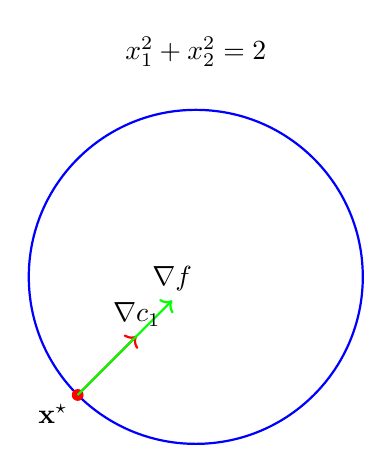
\begin{tikzpicture}[scale=1.5]
    % Circle constraint
    \draw[thick, blue] (0,0) circle (1.414);
    % Gradient vectors at solution
    \fill[red] (-1,-1) circle (0.05);
    \draw[->, red, thick] (-1,-1) -- (-0.5,-0.5);
    \draw[->, green, thick] (-1,-1) -- (-0.2,-0.2);
    % Labels
    \node[below left] at (-1,-1) {$\mathbf{x}^{\star}$};
    \node[above] at (-0.5,-0.5) {$\nabla c_1$};
    \node[above] at (-0.2,-0.2) {$\nabla f$};
    % Constraint equation
    \node[above] at (0,1.7) {$x_1^2 + x_2^2 = 2$};
  \end{tikzpicture}
\end{frame}

\begin{frame}{Optimality Condition for Equality Constraints}
  \begin{block}{Necessary Condition}
    At solution $\mathbf{x}^{\star}$, there exists $\lambda_1^{\star}$ such that:
    $$\nabla f(\mathbf{x}^{\star}) = \lambda_1^{\star} \nabla c_1(\mathbf{x}^{\star})$$
  \end{block}
  
  \textbf{Intuition:}
  \begin{itemize}
    \item For feasible descent direction $\mathbf{d}$: $\nabla c_1(\mathbf{x})^T \mathbf{d} = 0$ (stay on constraint)
    \item For improvement: $\nabla f(\mathbf{x})^T \mathbf{d} < 0$
    \item No such $\mathbf{d}$ exists when gradients are parallel
  \end{itemize}
  
  \vspace{0.3cm}
  \textbf{Lagrangian formulation:}
  $$\mathcal{L}(\mathbf{x}, \lambda_1) = f(\mathbf{x}) - \lambda_1 c_1(\mathbf{x})$$
  $$\nabla_{\mathbf{x}} \mathcal{L}(\mathbf{x}^{\star}, \lambda_1^{\star}) = \mathbf{0}$$
\end{frame}


% Problem 1
\begin{frame}
\frametitle{Exercise 1}
\begin{block}{Problem Statement}
\textbf{Minimize:} $f(x_1, x_2) = x_1 x_2$

\textbf{Subject to:} $x_1^2 + x_2^2 = 8$
\end{block}

\vspace{1cm}
Find the minimum value and the point(s) where it occurs.
\end{frame}

% Solution 1
\begin{frame}[allowframebreaks]
\frametitle{Solution to Exercise 1}

\textbf{Step 1: Set up the Lagrangian}
$$L(x_1, x_2, \lambda) = x_1 x_2 + \lambda(x_1^2 + x_2^2 - 8)$$

\textbf{Step 2: First-order conditions}
\begin{align}
\frac{\partial L}{\partial x_1} &= x_2 + 2\lambda x_1 = 0 \quad (1)\\
\frac{\partial L}{\partial x_2} &= x_1 + 2\lambda x_2 = 0 \quad (2)\\
\frac{\partial L}{\partial \lambda} &= x_1^2 + x_2^2 - 8 = 0 \quad (3)
\end{align}

\framebreak

\textbf{Step 3: Solve the system}

From equations (1) and (2):
\begin{align}
x_2 &= -2\lambda x_1\\
x_1 &= -2\lambda x_2
\end{align}

Substituting: $x_1 = -2\lambda(-2\lambda x_1) = 4\lambda^2 x_1$

If $x_1 \neq 0$: $1 = 4\lambda^2 \Rightarrow \lambda = \pm\frac{1}{2}$

\framebreak

\textbf{Case 1:} $\lambda = \frac{1}{2}$
\begin{itemize}
\item $x_2 = -x_1$
\item From constraint: $x_1^2 + x_1^2 = 8 \Rightarrow x_1 = \pm 2\sqrt{2}$
\item Critical points: $(2\sqrt{2}, -2\sqrt{2})$ and $(-2\sqrt{2}, 2\sqrt{2})$
\end{itemize}

\textbf{Case 2:} $\lambda = -\frac{1}{2}$
\begin{itemize}
\item $x_2 = x_1$
\item From constraint: $2x_1^2 = 8 \Rightarrow x_1 = \pm 2$
\item Critical points: $(2, 2)$ and $(-2, -2)$
\end{itemize}

\framebreak

\textbf{Step 4: Evaluate the objective function}

At $(2\sqrt{2}, -2\sqrt{2})$ and $(-2\sqrt{2}, 2\sqrt{2})$:
$$f = (2\sqrt{2})(-2\sqrt{2}) = -8$$

At $(2, 2)$ and $(-2, -2)$:
$$f = (2)(2) = 4$$

\vspace{0.5cm}
\begin{block}{Answer}
\textbf{Minimum value:} $-8$

\textbf{Occurs at:} $(2\sqrt{2}, -2\sqrt{2})$ and $(-2\sqrt{2}, 2\sqrt{2})$
\end{block}

\end{frame}

Problem 2
\begin{frame}
\frametitle{Exercise 2}
\begin{block}{Problem Statement}
\textbf{Minimize:} $f(x_1, x_2, x_3) = x_1^2 + x_2^2 + x_3^2$

\textbf{Subject to:} 
\begin{align}
g_1: \quad & x_1 + x_2 + x_3 = 6\\
g_2: \quad & x_1 - x_2 = 2
\end{align}
\end{block}

\vspace{1cm}
Find the minimum value and the point where it occurs.
\end{frame}

% Solution 2
\begin{frame}[allowframebreaks]
\frametitle{Solution to Exercise 2}

\textbf{Step 1: Set up the Lagrangian}
$$L = x_1^2 + x_2^2 + x_3^2 + \lambda_1(x_1 + x_2 + x_3 - 6) + \lambda_2(x_1 - x_2 - 2)$$

\textbf{Step 2: First-order conditions}
\begin{align}
\frac{\partial L}{\partial x_1} &= 2x_1 + \lambda_1 + \lambda_2 = 0 \quad (1)\\
\frac{\partial L}{\partial x_2} &= 2x_2 + \lambda_1 - \lambda_2 = 0 \quad (2)\\
\frac{\partial L}{\partial x_3} &= 2x_3 + \lambda_1 = 0 \quad (3)\\
\frac{\partial L}{\partial \lambda_1} &= x_1 + x_2 + x_3 - 6 = 0 \quad (4)\\
\frac{\partial L}{\partial \lambda_2} &= x_1 - x_2 - 2 = 0 \quad (5)
\end{align}

\framebreak

\textbf{Step 3: Solve for variables in terms of multipliers}

From the first-order conditions:
\begin{align}
x_3 &= -\frac{\lambda_1}{2} \quad \text{from (3)}\\
x_1 &= -\frac{\lambda_1 + \lambda_2}{2} \quad \text{from (1)}\\
x_2 &= -\frac{\lambda_1 - \lambda_2}{2} \quad \text{from (2)}
\end{align}

\framebreak

\textbf{Step 4: Use constraints to find multipliers}

From constraint (5): $x_1 - x_2 = 2$
$$-\frac{\lambda_1 + \lambda_2}{2} - \left(-\frac{\lambda_1 - \lambda_2}{2}\right) = 2$$
$$-\frac{\lambda_2}{} = 2 \Rightarrow \lambda_2 = -2$$

From constraint (4): $x_1 + x_2 + x_3 = 6$
$$-\frac{\lambda_1 + \lambda_2}{2} - \frac{\lambda_1 - \lambda_2}{2} - \frac{\lambda_1}{2} = 6$$
$$-\frac{3\lambda_1}{2} = 6 \Rightarrow \lambda_1 = -4$$

\framebreak

\textbf{Step 5: Find the solution}

With $\lambda_1 = -4$ and $\lambda_2 = -2$:
\begin{align}
x_1 &= -\frac{(-4) + (-2)}{2} = 3\\
x_2 &= -\frac{(-4) - (-2)}{2} = 1\\
x_3 &= -\frac{(-4)}{2} = 2
\end{align}

\textbf{Verification:} $3 + 1 + 2 = 6$ and $3 - 1 = 2$ 

\vspace{0.5cm}
\begin{block}{Answer}
\textbf{Minimum value:} $3^2 + 1^2 + 2^2 = 14$

\textbf{Occurs at:} $(3, 1, 2)$
\end{block}

\end{frame}


\subsection{A Single Inequality Constraint}
\begin{frame}{Example 2: Single Inequality Constraint}
  \begin{block}{Problem}
    $$\min x_1 + x_2 \quad \text{subject to} \quad 2 - x_1^2 - x_2^2 \geq 0$$
  \end{block}
  
  \begin{itemize}
    \item \textbf{Feasible set:} Disk of radius $\sqrt{2}$ (circle + interior)
    \item \textbf{Solution:} $\mathbf{x}^{\star} = (-1, -1)^T$ (same as before)
    \item \textbf{Key difference:} Sign of Lagrange multiplier matters
  \end{itemize}
  
  \vspace{0.3cm}
  % Placeholder for TikZ visualization
  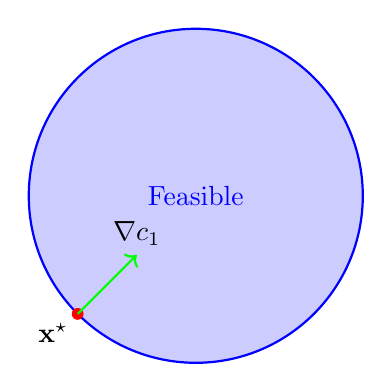
\begin{tikzpicture}[scale=1.5]
    % Filled circle (feasible region)
    \fill[blue!20] (0,0) circle (1.414);
    \draw[thick, blue] (0,0) circle (1.414);
    % Solution point
    \fill[red] (-1,-1) circle (0.05);
    \node[below left] at (-1,-1) {$\mathbf{x}^{\star}$};
    % Constraint normal pointing inward
    \draw[->, green, thick] (-1,-1) -- (-0.5,-0.5);
    \node[above] at (-0.5,-0.5) {$\nabla c_1$};
    % Feasible region label
    \node at (0,0) {\textcolor{blue}{Feasible}};
  \end{tikzpicture}
\end{frame}

\begin{frame}{Two Cases for Inequality Constraints}
  \textbf{Case I: Interior point} ($c_1(\mathbf{x}) > 0$)
  \begin{itemize}
    \item Constraint not restrictive
    \item Necessary condition: $\nabla f(\mathbf{x}) = \mathbf{0}$
    \item Lagrange multiplier: $\lambda_1 = 0$
  \end{itemize}
  
  \vspace{0.5cm}
  \textbf{Case II: Boundary point} ($c_1(\mathbf{x}) = 0$)
  \begin{itemize}
    \item Constraint is active
    \item Feasible descent direction $\mathbf{d}$: $\nabla c_1(\mathbf{x})^T \mathbf{d} \geq 0$
    \item No such direction when: $\nabla f(\mathbf{x}) = \lambda_1 \nabla c_1(\mathbf{x})$ with $\lambda_1 \geq 0$
  \end{itemize}
  
  \vspace{0.5cm}
  \begin{block}{Complementarity Condition}
    $$\lambda_1 c_1(\mathbf{x}) = 0$$
  \end{block}
\end{frame}

\subsection{Two Inequality Constraints}
\begin{frame}{Example 3: Two Inequality Constraints}
  \begin{block}{Problem}
    $$\min x_1 + x_2 \quad \text{subject to} \quad 2 - x_1^2 - x_2^2 \geq 0, \quad x_2 \geq 0$$
  \end{block}
  
  \begin{itemize}
    \item \textbf{Feasible set:} Half-disk
    \item \textbf{Solution:} $\mathbf{x}^{\star} = (-\sqrt{2}, 0)^T$
    \item \textbf{Both constraints active} at solution
  \end{itemize}
  
  \vspace{0.3cm}
  % Placeholder for TikZ visualization
  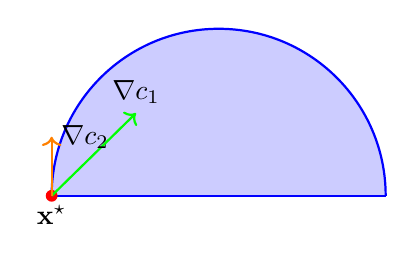
\begin{tikzpicture}[scale=1.5]
    % Half disk (feasible region)
    \fill[blue!20] (0,0) -- (1.414,0) arc (0:180:1.414) -- cycle;
    \draw[thick, blue] (-1.414,0) arc (180:0:1.414);
    \draw[thick, blue] (-1.414,0) -- (1.414,0);
    % Solution point
    \fill[red] (-1.414,0) circle (0.05);
    \node[below] at (-1.414,0) {$\mathbf{x}^{\star}$};
    % Constraint gradients
    \draw[->, green, thick] (-1.414,0) -- (-0.7,0.7);
    \draw[->, orange, thick] (-1.414,0) -- (-1.414,0.5);
    \node[above] at (-0.7,0.7) {$\nabla c_1$};
    \node[right] at (-1.414,0.5) {$\nabla c_2$};
  \end{tikzpicture}
\end{frame}

\begin{frame}{Multiple Constraints: KKT Conditions Preview}
  \textbf{Lagrangian:}
  $$\mathcal{L}(\mathbf{x}, \boldsymbol{\lambda}) = f(\mathbf{x}) - \lambda_1 c_1(\mathbf{x}) - \lambda_2 c_2(\mathbf{x})$$
  
  \textbf{Optimality conditions:}
  \begin{align}
    \nabla_{\mathbf{x}} \mathcal{L}(\mathbf{x}^{\star}, \boldsymbol{\lambda}^{\star}) &= \mathbf{0} \\
    \lambda_i^{\star} &\geq 0 \quad \text{for all } i \in \mathcal{I} \\
    \lambda_i^{\star} c_i(\mathbf{x}^{\star}) &= 0 \quad \text{for all } i
  \end{align}
  
  \vspace{0.3cm}
  \textbf{For Example 3:} $\boldsymbol{\lambda}^{\star} = (1/(2\sqrt{2}), 1)^T$
\end{frame}

\section{First-Order Optimality Conditions}
\subsection{Statement of First-Order Necessary Conditions}
\begin{frame}{Active Set and Constraint Qualification}
  \begin{definition}[Active Set]
    $$\mathcal{A}(\mathbf{x}) = \mathcal{E} \cup \{i \in \mathcal{I} \mid c_i(\mathbf{x}) = 0\}$$
  \end{definition}
  
  \begin{definition}[Linear Independence Constraint Qualification (LICQ)]
    At point $\mathbf{x}^{\star}$, LICQ holds if the set of active constraint gradients $\{\nabla c_i(\mathbf{x}^{\star}), i \in \mathcal{A}(\mathbf{x}^{\star})\}$ is linearly independent.
  \end{definition}
  
  \vspace{0.5cm}
  \textbf{Purpose:} Ensures constraint gradients are well-behaved and don't vanish inappropriately.
\end{frame}

\begin{frame}{Karush-Kuhn-Tucker (KKT) Conditions}
  \begin{theorem}[First-Order Necessary Conditions]
    If $\mathbf{x}^{\star}$ is a local solution and LICQ holds at $\mathbf{x}^{\star}$, then there exists $\boldsymbol{\lambda}^{\star}$ such that:
    \begin{align}
      \nabla_{\mathbf{x}} \mathcal{L}(\mathbf{x}^{\star}, \boldsymbol{\lambda}^{\star}) &= \mathbf{0} \tag{Stationarity}\\
      c_i(\mathbf{x}^{\star}) &= 0, \quad i \in \mathcal{E} \tag{Equality feasibility}\\
      c_i(\mathbf{x}^{\star}) &\geq 0, \quad i \in \mathcal{I} \tag{Inequality feasibility}\\
      \lambda_i^{\star} &\geq 0, \quad i \in \mathcal{I} \tag{Dual feasibility}\\
      \lambda_i^{\star} c_i(\mathbf{x}^{\star}) &= 0, \quad i \in \mathcal{E} \cup \mathcal{I} \tag{Complementarity}
    \end{align}
  \end{theorem}
  
  \begin{block}{General Lagrangian}
    $$\mathcal{L}(\mathbf{x}, \boldsymbol{\lambda}) = f(\mathbf{x}) - \sum_{i \in \mathcal{E} \cup \mathcal{I}} \lambda_i c_i(\mathbf{x})$$
  \end{block}
\end{frame}

\begin{frame}{KKT Conditions: Interpretation}
  \textbf{Stationarity:} $\nabla f(\mathbf{x}^{\star}) = \sum_{i \in \mathcal{A}(\mathbf{x}^{\star})} \lambda_i^{\star} \nabla c_i(\mathbf{x}^{\star})$
  \begin{itemize}
    \item Objective gradient is linear combination of active constraint gradients
  \end{itemize}
  
  \textbf{Complementarity:} $\lambda_i^{\star} c_i(\mathbf{x}^{\star}) = 0$
  \begin{itemize}
    \item Either constraint is active ($c_i = 0$) or multiplier is zero ($\lambda_i = 0$)
    \item Cannot have both $c_i > 0$ and $\lambda_i > 0$
  \end{itemize}
  
  \textbf{Dual feasibility:} $\lambda_i^{\star} \geq 0$ for inequality constraints
  \begin{itemize}
    \item Sign restriction crucial for inequality constraints
    \item No sign restriction for equality constraint multipliers
  \end{itemize}
\end{frame}

\subsection{Sensitivity}
\begin{frame}{Economic Interpretation of Lagrange Multipliers}
  \textbf{Sensitivity analysis:} How does optimal value change when constraints are perturbed?
  
  \vspace{0.3cm}
  Consider perturbed constraint: $c_i(\mathbf{x}) \geq -\epsilon \|\nabla c_i(\mathbf{x}^{\star})\|$
  
  \begin{block}{Key Result}
    $$\frac{df(\mathbf{x}^{\star}(\epsilon))}{d\epsilon} = -\lambda_i^{\star} \|\nabla c_i(\mathbf{x}^{\star})\|$$
  \end{block}
  
  \textbf{Interpretation:}
  \begin{itemize}
    \item $\lambda_i^{\star}$ measures sensitivity of optimal value to constraint $i$
    \item Large $\lambda_i^{\star}$ $\Rightarrow$ constraint $i$ is "tight" or "binding"
    \item $\lambda_i^{\star} = 0$ $\Rightarrow$ constraint $i$ has little impact on optimal value
  \end{itemize}
\end{frame}

\begin{frame}{Strongly vs. Weakly Active Constraints}
  \begin{definition}[Strongly Active Constraints]
    Inequality constraint $c_i$ is \textbf{strongly active} if $i \in \mathcal{A}(\mathbf{x}^{\star})$ and $\lambda_i^{\star} > 0$.
  \end{definition}
  
  \begin{definition}[Weakly Active Constraints]
    Inequality constraint $c_i$ is \textbf{weakly active} if $i \in \mathcal{A}(\mathbf{x}^{\star})$ and $\lambda_i^{\star} = 0$.
  \end{definition}
  
  \vspace{0.5cm}
  \textbf{Economic interpretation:}
  \begin{itemize}
    \item \textbf{Strongly active:} Relaxing constraint would improve objective
    \item \textbf{Weakly active:} Small constraint relaxation has no first-order effect
  \end{itemize}
\end{frame}

\section{Derivation of First-Order Conditions}
\subsection{Feasible Sequences}
\begin{frame}{Feasible Sequences Approach}
  \begin{definition}[Feasible Sequence]
    Given feasible point $\mathbf{x}^{\star}$, sequence $\{\mathbf{z}_k\}$ is feasible if:
    \begin{enumerate}
      \item $\mathbf{z}_k \neq \mathbf{x}^{\star}$ for all $k$
      \item $\lim_{k \to \infty} \mathbf{z}_k = \mathbf{x}^{\star}$  
      \item $\mathbf{z}_k$ is feasible for all $k$ sufficiently large
    \end{enumerate}
  \end{definition}
  
  \begin{definition}[Limiting Direction]
    Vector $\mathbf{d}$ is a limiting direction if:
    $$\lim_{k \to \infty} \frac{\mathbf{z}_k - \mathbf{x}^{\star}}{\|\mathbf{z}_k - \mathbf{x}^{\star}\|} = \mathbf{d}$$
    for some feasible sequence $\{\mathbf{z}_k\}$.
  \end{definition}
\end{frame}

\begin{frame}{First-Order Necessary Condition via Feasible Sequences}
  \begin{theorem}[Feasible Sequence Necessary Condition]
    If $\mathbf{x}^{\star}$ is a local solution, then for all feasible sequences $\{\mathbf{z}_k\}$ and their limiting directions $\mathbf{d}$:
    $$\nabla f(\mathbf{x}^{\star})^T \mathbf{d} \geq 0$$
  \end{theorem}
  
  \textbf{Proof idea:}
  \begin{itemize}
    \item If $\nabla f(\mathbf{x}^{\star})^T \mathbf{d} < 0$, then by Taylor expansion:
    $$f(\mathbf{z}_k) = f(\mathbf{x}^{\star}) + \|\mathbf{z}_k - \mathbf{x}^{\star}\| \mathbf{d}^T \nabla f(\mathbf{x}^{\star}) + o(\|\mathbf{z}_k - \mathbf{x}^{\star}\|)$$
    \item For large $k$: $f(\mathbf{z}_k) < f(\mathbf{x}^{\star})$ contradicting optimality
  \end{itemize}
\end{frame}

\subsection{Characterizing Limiting Directions}
\begin{frame}{Linearized Feasible Directions}
  \begin{definition}[Linearized Feasible Directions]
    $$F_1 = \left\{\alpha \mathbf{d} \mid \alpha > 0, \begin{array}{l}
    \mathbf{d}^T \nabla c_i(\mathbf{x}^{\star}) = 0, \quad i \in \mathcal{E} \\
    \mathbf{d}^T \nabla c_i(\mathbf{x}^{\star}) \geq 0, \quad i \in \mathcal{A}(\mathbf{x}^{\star}) \cap \mathcal{I}
    \end{array}\right\}$$
  \end{definition}
  
  \begin{lemma}[Characterization of Limiting Directions]
    When LICQ holds:
    \begin{enumerate}
      \item Every limiting direction satisfies the conditions defining $F_1$
      \item Every direction in $F_1$ is a limiting direction of some feasible sequence
    \end{enumerate}
  \end{lemma}
  
  \textbf{Consequence:} Under LICQ, optimality requires $\nabla f(\mathbf{x}^{\star})^T \mathbf{d} \geq 0$ for all $\mathbf{d} \in F_1$.
\end{frame}

\subsection{Introducing Lagrange Multipliers}
\begin{frame}{From Geometry to Algebra}
  \begin{lemma}[Lagrange Multiplier Characterization]
    There is no direction $\mathbf{d} \in F_1$ with $\mathbf{d}^T \nabla f(\mathbf{x}^{\star}) < 0$ if and only if there exists $\boldsymbol{\lambda}$ such that:
    $$\nabla f(\mathbf{x}^{\star}) = \sum_{i \in \mathcal{A}(\mathbf{x}^{\star})} \lambda_i \nabla c_i(\mathbf{x}^{\star})$$
    with $\lambda_i \geq 0$ for $i \in \mathcal{A}(\mathbf{x}^{\star}) \cap \mathcal{I}$.
  \end{lemma}
  
  \textbf{Geometric intuition:}
  \begin{itemize}
    \item Objective gradient must lie in cone generated by active constraint gradients
    \item Farkas' lemma: Either system has solution or alternative system has solution
  \end{itemize}
\end{frame}

\section{Second-Order Conditions}
\begin{frame}{Need for Second-Order Analysis}
  \textbf{First-order conditions are not sufficient!}
  
  \vspace{0.3cm}
  Consider directions $\mathbf{w}$ where first-order information is inconclusive:
  $$\mathbf{w}^T \nabla f(\mathbf{x}^{\star}) = 0$$
  
  \textbf{Question:} Does moving along $\mathbf{w}$ increase or decrease $f$?
  
  \vspace{0.5cm}
  \begin{definition}[Critical Cone]
    $$F_2(\boldsymbol{\lambda}^{\star}) = \left\{\mathbf{w} \in F_1 \mid \nabla c_i(\mathbf{x}^{\star})^T \mathbf{w} = 0, \text{ all } i \in \mathcal{A}(\mathbf{x}^{\star}) \cap \mathcal{I} \text{ with } \lambda_i^{\star} > 0\right\}$$
  \end{definition}
  
  \textbf{Key property:} For $\mathbf{w} \in F_2(\boldsymbol{\lambda}^{\star})$: $\mathbf{w}^T \nabla f(\mathbf{x}^{\star}) = 0$
\end{frame}

\begin{frame}{Second-Order Necessary Conditions}
  \begin{theorem}[Second-Order Necessary Conditions]
    If $\mathbf{x}^{\star}$ is a local solution, LICQ holds, and $\boldsymbol{\lambda}^{\star}$ satisfies KKT conditions, then:
    $$\mathbf{w}^T \nabla_{\mathbf{x}\mathbf{x}} \mathcal{L}(\mathbf{x}^{\star}, \boldsymbol{\lambda}^{\star}) \mathbf{w} \geq 0 \quad \text{for all } \mathbf{w} \in F_2(\boldsymbol{\lambda}^{\star})$$
  \end{theorem}
  
  \begin{theorem}[Second-Order Sufficient Conditions]
    If $\mathbf{x}^{\star}$ is feasible, KKT conditions hold, and:
    $$\mathbf{w}^T \nabla_{\mathbf{x}\mathbf{x}} \mathcal{L}(\mathbf{x}^{\star}, \boldsymbol{\lambda}^{\star}) \mathbf{w} > 0 \quad \text{for all } \mathbf{w} \in F_2(\boldsymbol{\lambda}^{\star}), \mathbf{w} \neq \mathbf{0}$$
    then $\mathbf{x}^{\star}$ is a strict local solution.
  \end{theorem}
\end{frame}

\section{Second-Order Conditions and Projected Hessians}
\begin{frame}{Projected Hessian Matrices}
  When strict complementarity holds: $F_2(\boldsymbol{\lambda}^{\star}) = \text{Null}(\mathbf{A})$
  
  where $\mathbf{A} = [\nabla c_i(\mathbf{x}^{\star})]_{i \in \mathcal{A}(\mathbf{x}^{\star})}^T$
  
  \vspace{0.3cm}
  Let $\mathbf{Z}$ be matrix whose columns span $\text{Null}(\mathbf{A})$.
  
  \begin{block}{Projected Hessian Conditions}
    \textbf{Necessary:} $\mathbf{Z}^T \nabla_{\mathbf{x}\mathbf{x}} \mathcal{L}(\mathbf{x}^{\star}, \boldsymbol{\lambda}^{\star}) \mathbf{Z} \succeq 0$
    
    \textbf{Sufficient:} $\mathbf{Z}^T \nabla_{\mathbf{x}\mathbf{x}} \mathcal{L}(\mathbf{x}^{\star}, \boldsymbol{\lambda}^{\star}) \mathbf{Z} \succ 0$
  \end{block}
  
  \vspace{0.3cm}
  \textbf{Computational approach:} Use QR factorization of $\mathbf{A}^T$ to find $\mathbf{Z}$.
\end{frame}

\begin{frame}{Summary: Characterizing Optimal Solutions}
  \begin{block}{Complete Characterization}
    Point $\mathbf{x}^{\star}$ is a local solution if:
    \begin{enumerate}
      \item \textbf{First-order:} KKT conditions hold
      \item \textbf{Second-order:} $\mathbf{w}^T \nabla_{\mathbf{x}\mathbf{x}} \mathcal{L}(\mathbf{x}^{\star}, \boldsymbol{\lambda}^{\star}) \mathbf{w} \geq 0$ for $\mathbf{w} \in F_2(\boldsymbol{\lambda}^{\star})$
    \end{enumerate}
  \end{block}

  
  \textbf{Practical verification:}
  \begin{itemize}
    \item Check LICQ (linear independence of active constraint gradients)
    \item Solve KKT system for $(\mathbf{x}^{\star}, \boldsymbol{\lambda}^{\star})$
    \item Verify projected Hessian conditions
  \end{itemize}
  
  \vspace{0.3cm}
  \textbf{Next:} Algorithms to find points satisfying these conditions!
\end{frame}



\begin{frame}{Constrained Optimization Problem}

\begin{block}{Exercise: 2D Optimization with Mixed Constraints}

\begin{align}
\text{minimize} \quad & f(x,y) = (x-2)^2 + (y-2)^2 \\
\text{subject to:} \quad & g(x,y) = x + y - 2 = 0 \quad \text{(equality)} \\
& h_1(x,y) = -x \leq 0 \quad \text{(i.e., } x \geq 0\text{)} \\
& h_2(x,y) = -y \leq 0 \quad \text{(i.e., } y \geq 0\text{)}
\end{align}

\vspace{0.3cm}
\textbf{Tasks:}
\begin{enumerate}
\item Write the Lagrangian function $L(x,y,\lambda,\mu_1,\mu_2)$
\item Implement gradient descent on the Lagrangian
\item Verify that $\mu_1^* = \mu_2^* = 0$ (inactive constraints)
\end{enumerate}
\end{block}

\begin{alertblock}{Geometric Interpretation}
Find the point closest to $(2,2)$ that lies on the line $x + y = 2$ and stays in the first quadrant.
\end{alertblock}

\end{frame}
\end{document}


